\gdef\ztexKeyValParent{}
\section{序言}\label{outer-toc:custom_file}
最后附上一些复杂的目录格式定制示例, 涵盖目录样式设置以及目录数据提取, 可作为用户深度定制的参考. 下面这段代码展示了后续样例会用
到的一些命令和依赖宏包:

\begin{dxample}[1]
% \usepackage{tikz}
% \usepackage{tikz-qtree}
% \usepackage[log]{tikz-qtree-patch}
% \usetikzlibrary { mindmap, trees }
\definecolor{SeaGreen}{rgb}{0.18, 0.55, 0.34}
\def\customtocthemecolor{SeaGreen}
\ExplSyntaxOn\makeatletter
\dim_new:N \linewidthfix
\def\tocupdatelinewidthfix{
  \dim_set:Nn \linewidthfix {\linewidth-2\fboxsep}
}
\def\ornamentcorner#1#2#3{
  \node[anchor=#1, rotate=#3, outer~sep=0pt, inner~sep=0pt] at (frame.#2)
  {\pgfornamenthan[width=.8cm, color=\customtocthemecolor]{10}};}
\def\ztochyperpage#1{\exp_args:Nne \hyper@link{link}{page.#1}{#1}}
\makeatother\ExplSyntaxOff
\end{dxample}



\section{测试数据}\label{ztoc-example-data} 本手册在排版目录时用到的测试数据: ``\texttt{data.toc}'', ``\texttt{data\_II.toc}'', ``\texttt{data.ptoc}''. \texttt{data.ptoc} 文件仅用于向读者展示 \pkg{sect} 模块中 keyval seq 的存储结构； 当 ``\texttt{dump-ptable = true}'' 时,
\ztex{} 会自动生成该文件.

\def\exampleUR{\texttt{data.toc}}
\begin{DocExample}[++]
\contentsline {section}{{1}{AAA-1}}{1}{}
\contentsline {subsection}{{1.1}{BBB-1}}{1}{}
\contentsline {subsubsection}{{1.1.1}{CCC-1}}{1}{}
\contentsline {subsubsection}{{1.1.2}{CCC-2}}{1}{}
\contentsline {subsubsection}{{1.1.3}{CCC-3}}{1}{}
\contentsline {subsubsection}{{1.1.4}{CCC-4}}{1}{}
\contentsline {subsubsection}{{1.1.5}{CCC-5}}{1}{}
\contentsline {subsection}{{1.2}{BBB-2}}{1}{}
\contentsline {subsubsection}{{1.2.1}{CCC-6}}{1}{}
\contentsline {subsubsection}{{1.2.2}{CCC-7}}{1}{}
\contentsline {subsubsection}{{1.2.3}{CCC-8}}{1}{}
\contentsline {subsubsection}{{1.2.4}{CCC-9}}{1}{}
\contentsline {subsection}{{1.3}{BBB-3}}{1}{}
\end{DocExample}


\def\exampleUR{\texttt{data\_II.toc}}
\begin{DocExample}[++]
\contentsline{section}{{1}{AAA-1}}{1}{}%
\contentsline{subsection}{{1}{BBB-1}}{1}{}%
\contentsline{subsubsection}{{1.1.1}{CCC-1}}{1}{}%
\contentsline{subsubsection}{{1.1.2}{CCC-2}}{2}{}%
\contentsline{subsubsection}{{1.1.3}{CCxxxC-3}}{3}{}%
\contentsline{subsubsection}{{1.1.4}{CCssgda\-shgfeC-4}}{100}{}%
\contentsline{subsubsection}{{1.1.5}{CsasfCC-5}}{123}{}%
\contentsline{subsubsection}{{1.1.6}{CasklklCC-x}}{999}{}%
\contentsline{subsection}{{2}{B   BB-2}}{1}{}%
\contentsline{subsubsection}{{1.2.1}{CCC-6}}{1}{}%
\end{DocExample}


\def\exampleUR{\texttt{data.ptoc}}
\begin{DocExample}[++]
class={section},name={1},title={AAA-1},page={1},anchor={section.1},raw={\contentsline {section}{{1}{AAA-1}}{1}{}}
class={subsection},name={1.1},title={BBB-1},page={1},anchor={subsection.1.1},raw={\contentsline {subsection}{{1.1}{BBB-1}}{1}{}}
class={subsubsection},name={1.1.1},title={CCC-1},page={1},anchor={subsubsection.1.1.1},raw={\contentsline {subsubsection}{{1.1.1}{CCC-1}}{1}{}}
class={subsubsection},name={1.1.2},title={CCC-2},page={1},anchor={subsubsection.1.1.2},raw={\contentsline {subsubsection}{{1.1.2}{CCC-2}}{1}{}}
class={subsubsection},name={1.1.3},title={CCC-3},page={1},anchor={subsubsection.1.1.3},raw={\contentsline {subsubsection}{{1.1.3}{CCC-3}}{1}{}}
class={subsubsection},name={1.1.4},title={CCC-4},page={1},anchor={subsubsection.1.1.4},raw={\contentsline {subsubsection}{{1.1.4}{CCC-4}}{1}{}}
class={subsubsection},name={1.1.5},title={CCC-5},page={1},anchor={subsubsection.1.1.5},raw={\contentsline {subsubsection}{{1.1.5}{CCC-5}}{1}{}}
class={subsection},name={1.2},title={BBB-2},page={1},anchor={subsection.1.2},raw={\contentsline {subsection}{{1.2}{BBB-2}}{1}{}}
class={subsubsection},name={1.2.1},title={CCC-6},page={1},anchor={subsubsection.1.2.1},raw={\contentsline {subsubsection}{{1.2.1}{CCC-6}}{1}{}}
class={subsubsection},name={1.2.2},title={CCC-7},page={1},anchor={subsubsection.1.2.2},raw={\contentsline {subsubsection}{{1.2.2}{CCC-7}}{1}{}}
class={subsubsection},name={1.2.3},title={CCC-8},page={1},anchor={subsubsection.1.2.3},raw={\contentsline {subsubsection}{{1.2.3}{CCC-8}}{1}{}}
class={subsubsection},name={1.2.4},title={CCC-9},page={1},anchor={subsubsection.1.2.4},raw={\contentsline {subsubsection}{{1.2.4}{CCC-9}}{1}{}}
class={subsection},name={1.3},title={BBB-3},page={1},anchor={subsection.1.3},raw={\contentsline {subsection}{{1.3}{BBB-3}}{1}{}}
\end{DocExample}
\resetExampleUR



\clearpage
\section{案例:1} 一个很简单的案例:

\begin{DocExample}*
\begingroup
\ztocformat\subsection
  {
    format+=\color{teal}, 
    leader.sep=1pt, 
    leader.raise=2.5pt, 
    page.width=10pt
  }
\ztocgroupinsert{subsection,1,begin}%
  {%
    \begin{framed}%
    \pgfornament[width = 2cm,color = teal]{67}%
    \qquad\rule[-5em]{.5pt}{10em}%
    \begin{minipage}{.75\linewidth}%
  }
\ztocgroupinsert{subsection,1,end}%
  {%
    \end{minipage}%
    \end{framed}%
  }
\zlocaltoc{subsection}{4}
\endgroup
\end{DocExample}

% \noindent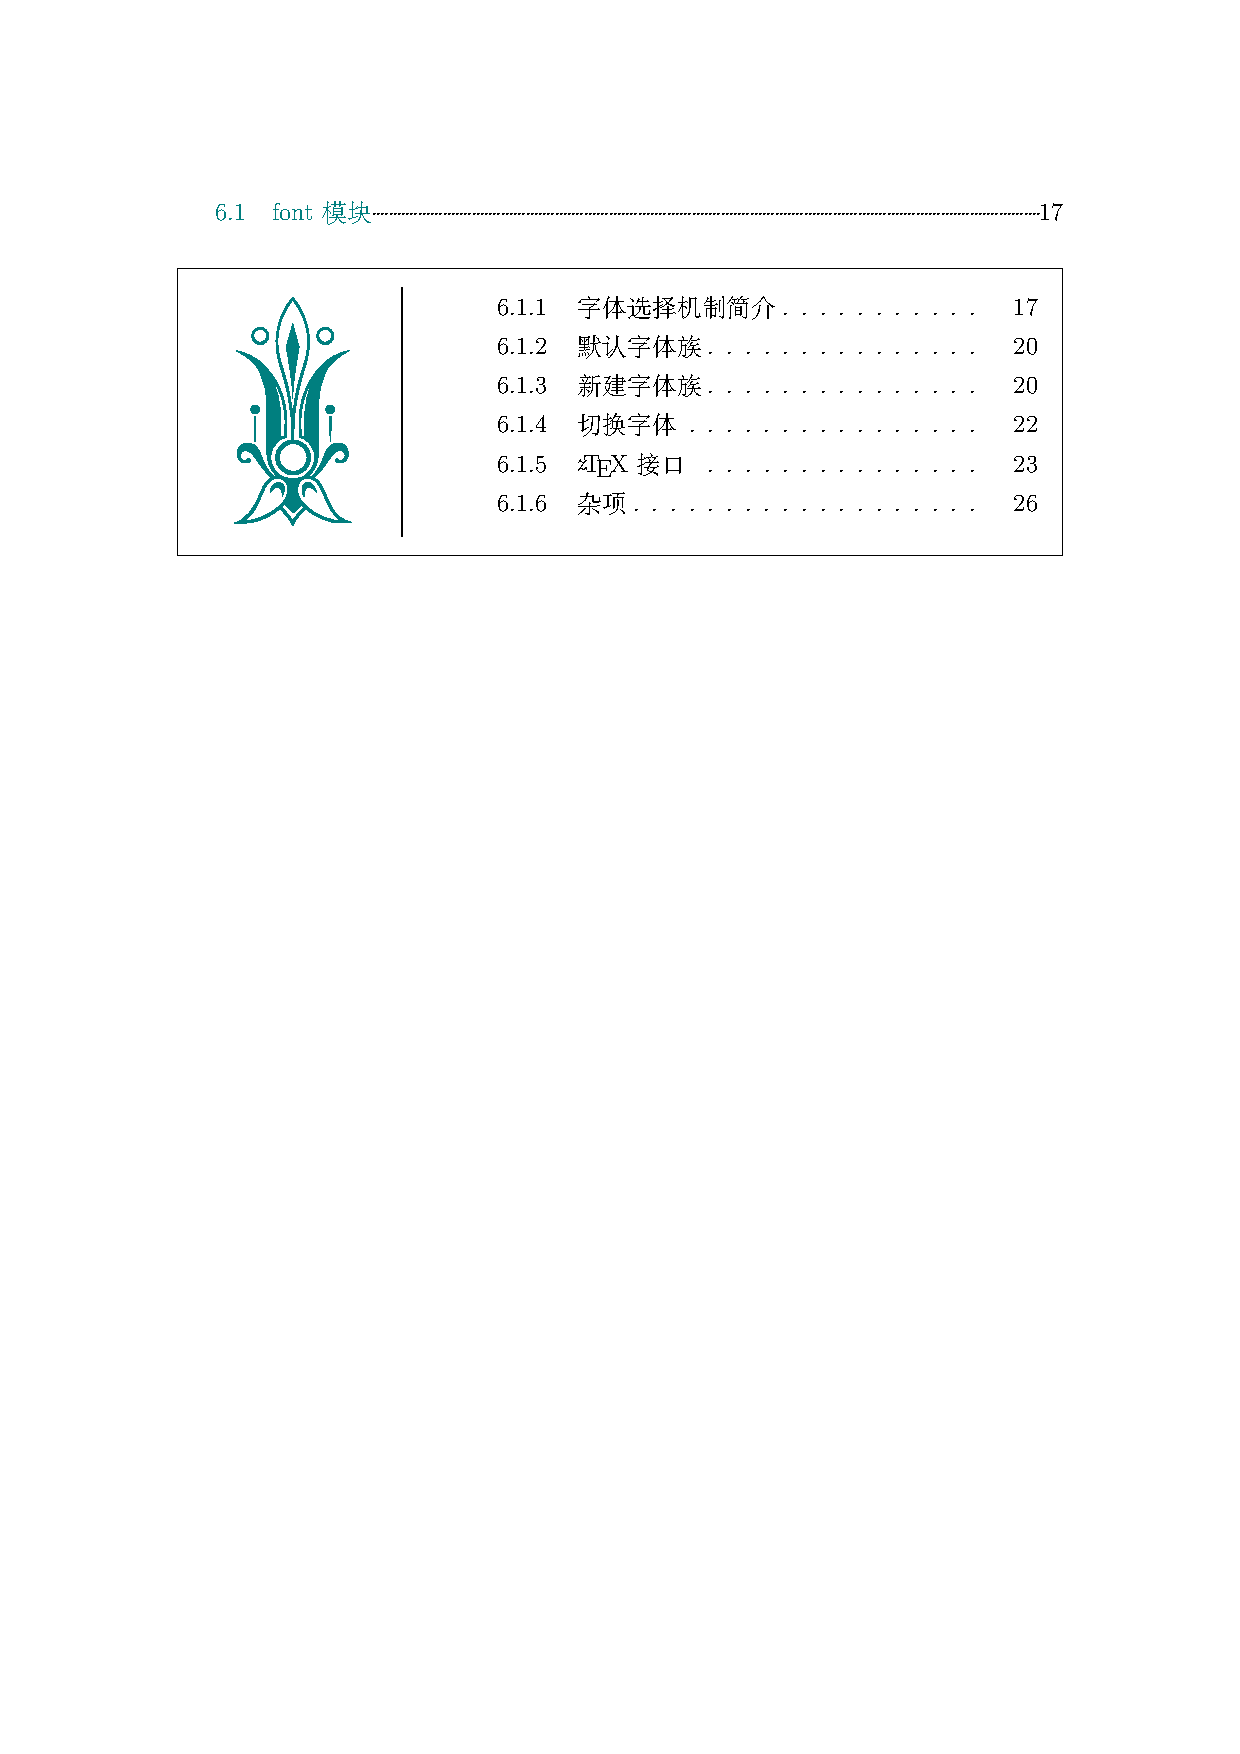
\includegraphics[width=\textwidth]{./support/pics/toc_group.pdf}

\section{案例:2}\label{ztoc:hook-position} 下面这个案例清晰地展示了目录中这些 
hook 的位置关系, \fbox{BG:\meta{int}} 和 \fbox{EG:\meta{int}} 代表目录条目自身
局部组的开始和结束位置(这些局部组目前已被移除 -- 2025-09-12).
\vskip1.25em\relax
\begin{DocExample}*[++]
\ExplSyntaxOn
\int_new:N \g__test_toc_group_int
\AddToHook{ztoc/tocline/begin}
  {
    \fbox{BG:\int_use:N \g__test_toc_group_int}
  }
\AddToHook{ztoc/tocline/end}
  {
    \fbox{EG:\int_use:N \g__test_toc_group_int}
    \int_gincr:N \g__test_toc_group_int
  }
\cs_new:Npn \__debug_ztoc_hook:nn #1#2
  { \ztocgroupinsert{#1}{\fbox{\color{#2}\sffamily #1}} }

% begin/end hooks:
\__debug_ztoc_hook:nn {subsection,1,begin}{red}
\__debug_ztoc_hook:nn {subsection,1,end}{red}
\__debug_ztoc_hook:nn {subsubsection,5,begin}{gray}
\__debug_ztoc_hook:nn {subsubsection,5,end}{gray}
% new before/after hooks:
\__debug_ztoc_hook:nn {subsection,1,before}{blue}
\__debug_ztoc_hook:nn {subsection,1,after}{blue}
\__debug_ztoc_hook:nn {subsubsection,1,before}{teal}
\__debug_ztoc_hook:nn {subsubsection,1,after}{teal}
\__debug_ztoc_hook:nn {subsubsection,3,before}{purple}
\__debug_ztoc_hook:nn {subsubsection,3,after}{purple}
\ExplSyntaxOff
\zlocaltoc{subsection}{4}
\end{DocExample}
\RemoveFromHook{ztoc/tocline/begin}
\RemoveFromHook{ztoc/tocline/end}


\clearpage
\section{案例:3} 这个案例相较之上一个案例更加复杂:

\begin{DocExample}*
\begingroup\makeatletter
\tocupdatelinewidthfix
\def\customtocthemecolor{teal}
\ztocformat\subsection
  {
    explicit=true,
    code={%
      \noindent\fcolorbox{white}{\customtocthemecolor}{\hb@xt@\linewidthfix
        {\bfseries\large\color{white}\ztocname
          \hskip.75em\relax\ztoctitle\hfill\ztocpage}}%
    }
  }
\ztocformat\subsubsection
  {
    format+=\color{\customtocthemecolor},
    page.format+=\color{\customtocthemecolor},
    name.before=\S\;
  }
\ztocgroupinsert{subsection,1,begin}%
  {%
    \begin{tcolorbox}[
      enhanced, sharp corners,
      boxrule=.5pt, colback=white,
      left=20pt, colframe=\customtocthemecolor,
      overlay={
        \ornamentcorner{north west}{north west}{0}
        \ornamentcorner{north west}{south west}{90}
        \ornamentcorner{north west}{south east}{180}
        \ornamentcorner{north west}{north east}{270}
      }
    ]
    \pgfornament[width = 2.5cm,color = \customtocthemecolor]{8}%
    \kern-6pt\relax\begin{minipage}{.75\linewidth}%
  }
\ztocgroupinsert{subsection,1,end}%
  {%
    \end{minipage}%
    \end{tcolorbox}%
  }
\zlocaltoc{subsection}{4}
\makeatother\endgroup
\end{DocExample}


\clearpage
\section{案例:4} 我们可以使用 \cmd{\ztocgroupinsert} 命令复刻 \pkg{titletoc}
宏包所提供的样式:

\begin{DocExample}*
\makeatletter
\def\customssstyle#1{%
  \ztocgroupinsert{subsection,#1,begin}
    {\raggedright\hangindent2.3em\relax\noindent\hskip2.3em\relax【}
  \ztocgroupinsert{subsection,#1,end}{】\par}
}
\makeatother
\customssstyle{1} \customssstyle{2}
\customssstyle{3} \customssstyle{4}
{
  \ztocformat\subsubsection{
    explicit=true,
    code={%
      \textit{\ztocname\enskip\ztoctitle\enskip
      (\ztochyperpage{\ztocpage})\ztociflast{}{;}\enskip}}
  }
  \ztocformat\subsection{
    explicit=true,
    code = {%
      \S\;\ztocname\enskip\ztoctitle
      \hskip1em\ztochyperpage{\ztocpage}\par}
  }
  \begin{multicols}{2}
    \zlocaltoc{subsection}{4, 11, 8, 6}
  \end{multicols}
}
\end{DocExample}



\clearpage
\setcounter{tocdepth}{3}
\section{案例: 5} 这个案例相较之上一个案例更加复杂:

\begin{DocExample}*
\begingroup\makeatletter
% \setcounter{tocdepth}{3}
\def\customtocthemecolor{SeaGreen}
\ztocformat\section
  {
    explicit=true,
    code={%
      \noindent\hskip1.5em\fcolorbox{white}{\customtocthemecolor}{\hb@xt@
        \dimexpr\linewidth-2\fboxsep-1.5em\relax
        {\bfseries\large\color{white}第\zhnumber{\ztocname}节
          \hskip.75em\relax\ztoctitle\hfill\ztocpage}}%
    }
  }
\ztocformat\subsection{
  name.before=\S\;, name.width=2.7em,
  format+=\color{\customtocthemecolor},
  page.format+=\color{\customtocthemecolor},
  leader.sep=2pt, page.width=1em,
  hyper.title=true,
  leader.content=\textcolor{\customtocthemecolor}{.},
}
\ztocgroupinsert{section,1,before}%
  {%
    \begin{tcolorbox}[
      enhanced, sharp corners,
      boxrule=.5pt, colback=white,
      left=20pt, colframe=\customtocthemecolor,
      overlay={
        \ornamentcorner{north west}{north west}{0}
        \ornamentcorner{north west}{south west}{90}
        \ornamentcorner{north west}{south east}{180}
        \ornamentcorner{north west}{north east}{270}
      }
    ]
    \pgfornament[width = 2.5cm,color = \customtocthemecolor]{10}%
    \begin{minipage}{.77\linewidth}%
  }
\ztocgroupinsert{section,1,begin}{%
  % \setlength{\columnsep}{0em}
  \begin{multicols}{2}}
\ztocgroupinsert{section,1,after}%
  {%
    \end{multicols}%
    \end{minipage}%
    \end{tcolorbox}%
  }
\zlocaltoc{section}{6}
\makeatother\endgroup
\end{DocExample}
\setcounter{tocdepth}{4}


\clearpage
\section{案例: 6}\label{toc-longtable} 这个案例复刻了 \pkg{etoc} 中的目录样式(参见 \pkg{etoc} 宏包第 39 节):

\begin{dxample}[1]
\ztocgroupinsert{section,1,before}
  {\begin{longtable}{|l|l|r|}}
\ztocgroupinsert{section,4,after}
  {\\ \hline\end{longtable}}
{
  \ztocformat\section{
    explicit=true,
    code = {%
      \ztociffirst{\kill\hline\multicolumn{3}{|c|}{\large\bfseries Table of Contents}\\\hline}{\\\hline}%
      \multicolumn{3}{||c||}{\bfseries 第\;\ztocname\;节\enskip\ztoctitle}%
    }
  }
  \ztocformat\subsection{
    explicit=true,
    code ={\\\hline
      \textbf{\S\ztocname} & \ztocname\enskip\ztoctitle & \ztochyperpage{\ztocpage}
    }
  }
  \ztocformat\subsubsection{
    explicit=true,
    code = {\\
      & \ztocname\enskip\ztoctitle & \ztochyperpage{\ztocpage}
    }
  }
  \zlocaltoc{section}{1, 2, 7, 9}
}
\end{dxample}


\clearpage
\section{案例: 7} 这个案例也是受到 \pkg{etoc} 宏包的启发 -- 将目录展示为思维导图的形式:

\begin{dxample}[1]
\definecolor{Green}{HTML}{15821b}
\tikzset{
  rootKey/.style={draw, rectangle, rounded corners, fill=Green, text=white},
}
\ExplSyntaxOn
\cs_new:Npn \__toc_tree:nn #1#2
  {
    \quark_if_no_value:nF {#1}
      {
        \Tree[.\node[rootKey]{#1};~#2 ]
      }
  }
\cs_generate_variant:Nn \__toc_tree:nn {oe}
\def\wraper#1{[.{\exp_not:n {#1}}~]}
\cs_new:Npn \ztoc_typeset_toctree:nnn #1#2#3
  {
    \ztoc_table_filter_key_byclass:nnnNN {#1}{#2}{#3}
      \g_ztoc_keyvaltoc_seq \g_tmpb_seq
    \seq_gpop_left:NN \g_tmpb_seq \secRoot
    \__toc_tree:oe { \secRoot }
      { \seq_map_function:NN \g_tmpb_seq \wraper }
  }
\def\TocTree#1#2#3
  {
    \exp_args:Nne \ztoc_typeset_toctree:nnn
      {#1}{#2}{#3}
  }
\ExplSyntaxOff

\noindent\begin{tikzpicture}[
    grow'=right,
    level distance=50pt,
    sibling distance=10pt,
    level 1/.style={level distance=25pt},
    every tree node/.style={anchor=west, draw, rectangle, rounded corners, fill=gray!25},
    every level 0 node/.style={anchor=east},
    edge from parent/.style={
      draw, thick, rounded corners,
      edge from parent path={
        (\tikzparentnode.east) -- +(10pt, 0pt)
        |- (\tikzchildnode.west)
      }
    },
  ]
  \TocTree{subsection}{4}{title}
  \begin{scope}[xshift=12cm]
    \TocTree{subsection}
      {\ztocindex{subsection}{\pkg{alias} 库}}
      {page}
  \end{scope}
\end{tikzpicture}
\end{dxample}


\clearpage
\section{案例: 8} 这个案列相较之上一个案例更加复杂, 它展示了 \cmd{\ztoc_group_parser:NNNnnnnn} 命令
中 \meta{step code} 的使用方法:

\begin{dxample}[0]
% \usetikzlibrary { mindmap, trees }
\ExplSyntaxOn
\int_new:N \g__mindmap_color_int
\seq_new:N \g__mindmap_data_seq
\seq_new:N \g__mindmap_keyvaldata_seq
\tl_new:N \g__mindmap_filter_data_tl
\def\toclinecmd#1#2#3#4
  {
    % override hyperlink color.
    {\ztexlink{#1.#2}{\textcolor{white}{#3(#4)}}}
  }
\cs_new:Npn \__ztoc_gen_mindmap_data:nn #1#2
  {
    \tl_gclear:N \g_tmpa_tl
    \ztoc_table_filter_byclass:nnNN
      { #1 }{ #2 } 
      \g_ztoc_keyvaltoc_seq
      \g__mindmap_data_seq
    \ztoc_generate_keyvaltable_seq:NN
      \g__mindmap_data_seq
      \g__mindmap_keyvaldata_seq
    \ztoc_group_parser:NNNnnnnn \g__mindmap_keyvaldata_seq
      \toclinecmd \g_tmpa_tl
        {
          child [ concept~color = blue!
            \int_eval:n{\g__mindmap_color_int*6}!green
          ] \bgroup node[concept]
        }
      {}{}{\egroup}{\int_gincr:N \g__mindmap_color_int}
    % replace '\bgroup' and '\egroup' by '{' and '}'. 
    \str_clear:N \l_tmpa_str
    \exp_args:NNo \str_set:Nn \l_tmpa_str { \g_tmpa_tl }
    \exp_args:NNne \str_replace_all:Nnn \l_tmpa_str
      { \bgroup }{ \char_generate:nn {123}{12} }
    \exp_args:NNne \str_replace_all:Nnn \l_tmpa_str
      { \egroup }{ \char_generate:nn {125}{12} }
    \tl_gset_rescan:Nno \g__mindmap_filter_data_tl
      { \cctab_select:N \c_document_cctab }
      { \l_tmpa_str }
  }
\cs_new:Npn \__tkz_mind_map:n #1
  {
    \tl_if_empty:nF {#1}
      {
        \node[concept] 
          {\color{white}\ztex{}~Interface}
          #1;
      }
  }
\newcommand{\mindmap}[2]
  {
    \__ztoc_gen_mindmap_data:nn
      { #1 }{ #2 }
    \exp_args:No \__tkz_mind_map:n
      { \g__mindmap_filter_data_tl }
  }
\ExplSyntaxOff
\begin{tikzpicture}[
    mindmap, grow cyclic,
    text width=2cm, align=flush center,
    nodes={concept}, concept color=blue!60,
    root concept/.append style={
      text width=4cm, font=\Large
    },
    level 1 concept/.append style={
      font=\normalsize, color=white
    },
    level 1/.append style={
      level distance=5cm, sibling angle=45,
      text width=3cm, font=\Large
    },
    level 2/.append style={
      level distance=9cm, sibling angle=90,
      text width=3cm, font=\Large
    },
    level 3/.append style={
      level distance=5cm, sibling angle=45,
      text width=3cm, font=\Large
    },
  ]
  \mindmap{section}{7}
\end{tikzpicture}
\end{dxample}


% NOTE: 1. for that this figure is too big,
%          we compile it manually.
%       2. these commands have been declared
%          in the cover page.
\newgeometry{margin=0pt}
\thispagestyle{empty}
\mbox{}\vfill
\ExplSyntaxOn
% \int_new:N \g__mindmap_color_int
% \seq_new:N \g__mindmap_data_seq
% \seq_new:N \g__mindmap_keyvaldata_seq
\def\toclinecmd#1#2#3#4
  {
    % override hyperlink color.
    {\ztexlink{#1.#2}{\textcolor{white}{#3(#4)}}}
  }

% \cs_new:Npn \__ztoc_gen_mindmap_data:nn #1#2
%   {
%     \ztoc_table_filter_byclass:nnNN
%       { #1 }{ #2 } 
%       \g_ztoc_keyvaltoc_seq
%       \g__mindmap_data_seq
%     \ztoc_generate_keyvaltable_seq:NN
%       \g__mindmap_data_seq
%       \g__mindmap_keyvaldata_seq
%     \ztoc_group_parser:NNNnnnnn \g__mindmap_keyvaldata_seq
%       \toclinecmd \g_tmpa_tl
%         {
%           child [ concept~color = blue!
%             \int_eval:n{\g__mindmap_color_int*6}!green
%           ] \bgroup node[concept]
%         }
%       {}{}{\egroup}{\int_gincr:N \g__mindmap_color_int}
%     % replace '\bgroup' and '\egroup' by '{' and '}'. 
%     \exp_args:NNo \str_set:Nn \l_tmpa_str { \g_tmpa_tl }
%     \exp_args:NNne \str_replace_all:Nnn \l_tmpa_str
%       { \bgroup }{ \char_generate:nn {123}{12} }
%     \exp_args:NNne \str_replace_all:Nnn \l_tmpa_str
%       { \egroup }{ \char_generate:nn {125}{12} }
%     \tl_gset_rescan:Nno \g_tmpa_tl
%       { \cctab_select:N \c_document_cctab }
%       { \l_tmpa_str }
%   }
% \cs_new:Npn \__tkz_mind_map:n #1
%   {
%     \tl_if_empty:nF {#1}
%       {
%         \node[concept] 
%           {\color{white}\ztex{}~Interface}
%           #1;
%       }
%   }
\newcommand{\mindmapAFTER}[2]
  {
    % \__ztoc_gen_mindmap_data:nn
    %   { #1 }{ #2 }
    \exp_args:No \__tkz_mind_map:n
      { \g__mindmap_filter_data_tl }
  }
\ExplSyntaxOff
\noindent\begin{tikzpicture}[
    mindmap, grow cyclic,
    text width=2cm, align=flush center,
    nodes={concept}, concept color=blue!60,
    root concept/.append style={text width=4cm, font=\Large},
    level 1/.append style={level distance=5cm, sibling angle=45, text width=3cm, font=\Large},
    level 2/.append style={level distance=8.75cm, sibling angle=90, text width=3cm, font=\Large},
    level 3/.append style={level distance=5cm, sibling angle=45, text width=3cm, font=\Large},
    level 1 concept/.append style={font=\normalsize, color=white},
  ]
  \mindmapAFTER{section}{7}
\end{tikzpicture}
\vfill\mbox{}
\restoregeometry


% \clearpage
\newgeometry{left=2.5cm, right=2.5cm}
\section{案例: 9} 下面这个案例展示了 \cmd{\ztociffirst}, \cmd{\ztociflast} 以及 \cmd{\ztocdepth}
等命令的使用方法:

\begin{dxample}[0]
\ExplSyntaxOn
\newcommand{\nbraket}
  { \makebox[0pt]{\rule[-7.5pt]{.75pt}{19pt}} }
\newcommand{\ubraket}
  {
    \makebox[0pt]{
      \rule[-7pt]{.75pt}{10pt}
    }
    \makebox[0pt][l]{
      \kern-.375pt\raise3pt\hbox{\rule{3pt}{.75pt}}
    }
  }
\newcommand{\bbraket}
  {
    \makebox[0pt]{ \rule[3pt]{.75pt}{10pt} }
    \makebox[0pt][l]
      { \kern-.375pt\raise3pt
      \hbox{\rule{3pt}{.75pt}} }
  }
\newcommand{\showbar}
  {
    \prg_replicate:nn {\ztocdepth - 2}
      { \kern20pt \nbraket }
    \kern20pt \ztociffirst { \ubraket }
      { \ztociflast{\bbraket}{\nbraket} }
  }
\ztocformat{\section, \subsection, \subsubsection}
  {
    explicit=true,
    code = {
      \noindent
      \prg_replicate:nn {\ztocdepth-1}
        {
          \hskip 20pt\relax
        }
      \llap{\smash{\showbar}}
      \kern10pt
      \ztoctitle\par
    }
  }
\ExplSyntaxOff
{
  \ztocformat\subsection{ignore.name={10.}}
  \ztocformat\subsubsection{ignore.name={10.}}
  \multicolcontents{2}
}
\end{dxample}

\newgeometry{margin=0pt}
\thispagestyle{empty}
\begin{center}
  \mbox{}\vfill
  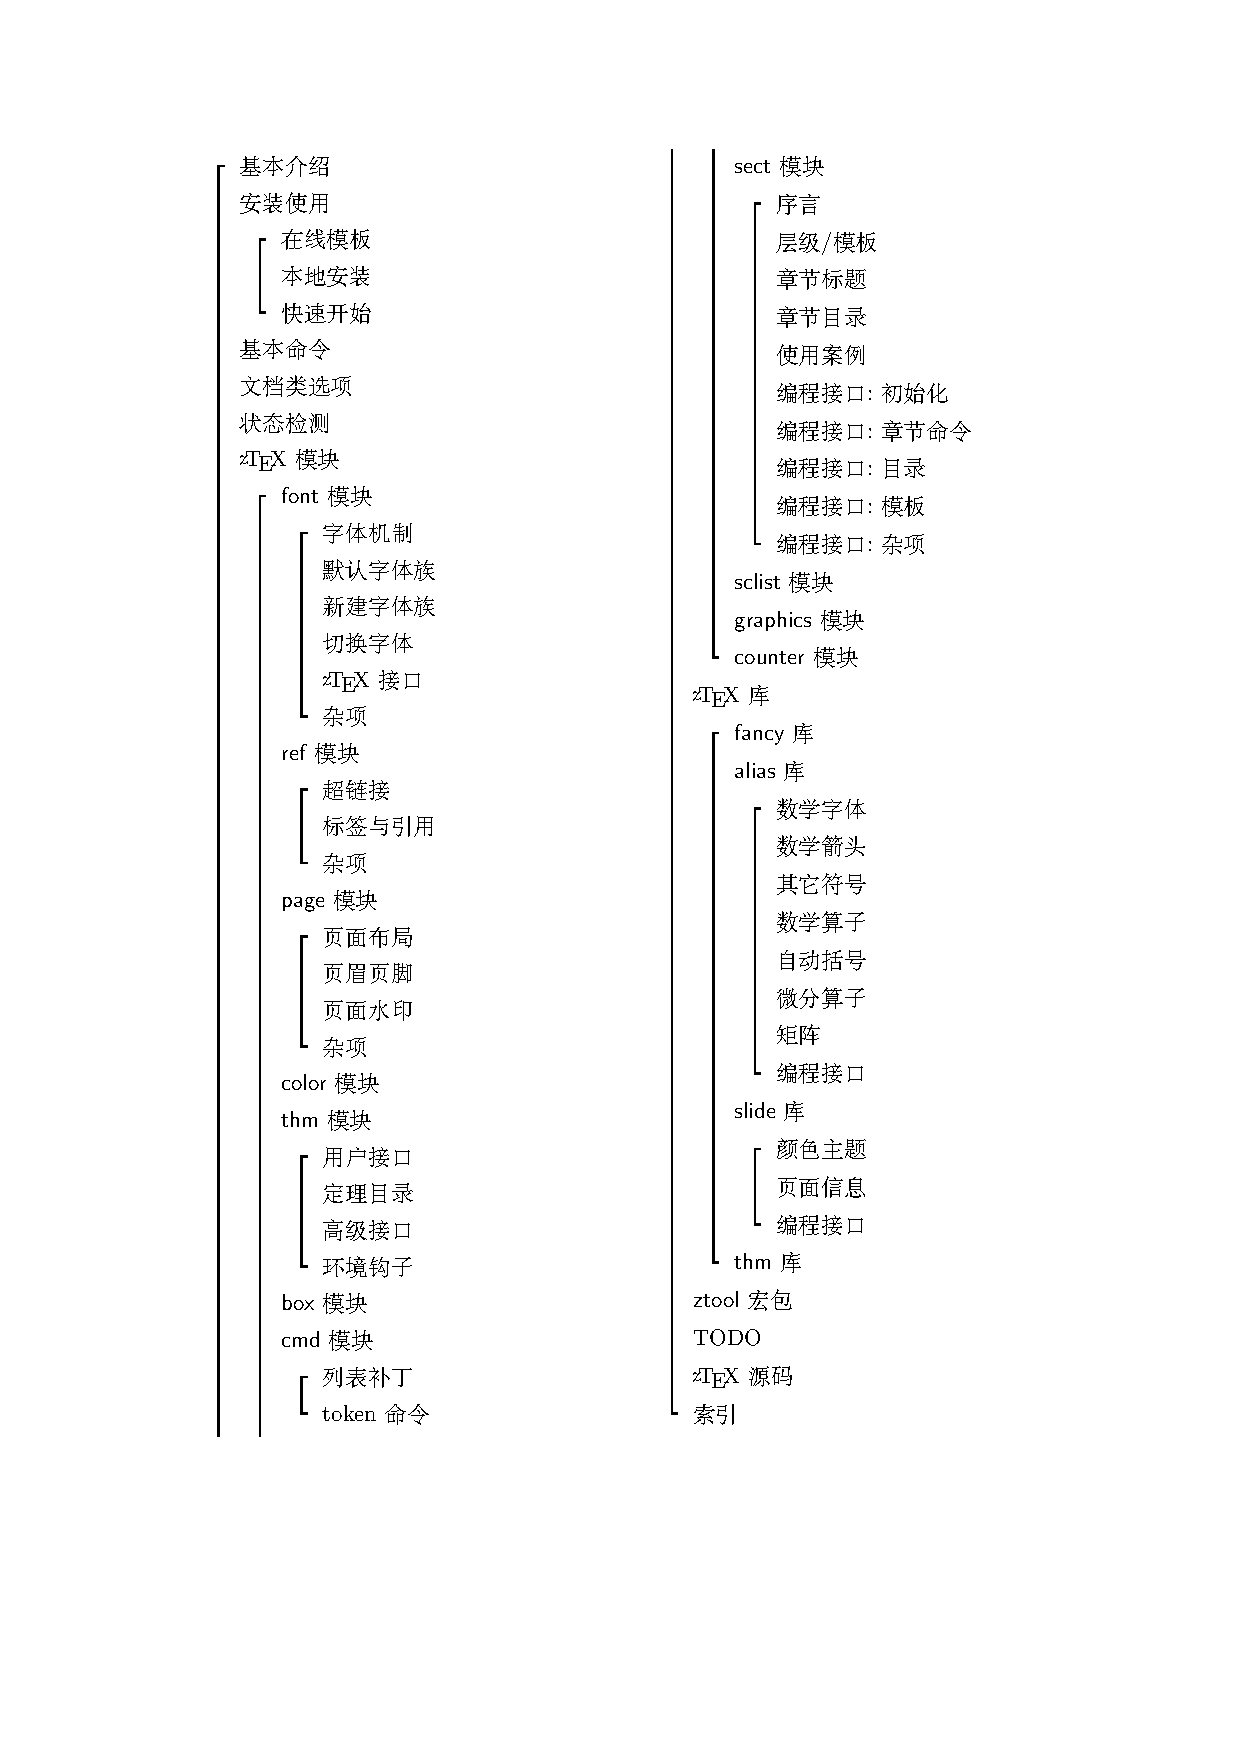
\includegraphics[height=.95\paperheight]{./support/pics/toclevel.pdf}
  \vfill\mbox{}
\end{center}
\restoregeometry


\newgeometry{left=2.5cm, right=2.5cm}
\section{案例: 10} 下面这个案例相较之上一个案例更加复杂, 但它展示了 \cmd{\ztoc_group_parser:NNNnnnnn} 命令的
强大和普适性:

\begin{dxample}[0]
% \usepackage{tikz}
% \usepackage{tikz-qtree}
% \usepackage{tikz-qtree-patch}
\definecolor{Red}{HTML}{e32b2d}
\definecolor{Green}{HTML}{15821b}
\definecolor{Blue}{HTML}{0984e3}
\tikzset{
  section/.style={draw, rectangle, rounded corners, fill=Red},
  subsection/.style={draw, rectangle, rounded corners, fill=Blue, text=white},
  subsubsection/.style={draw, rectangle, rounded corners, fill=Green, text=white},
}
\ExplSyntaxOn
% \def\toclinecmd#1#2#3#4{{#1:#2:#3:#4}~}
\def\toclinecmd#1#2#3#4{{\gparserclass(\gparserindex):#2:#3:#4}~}
\ztoc_group_parser:NNNnnnnn \g_ztoc_keyvaltoc_seq
  \toclinecmd \g_tmpa_tl {[.}{}{}{~]}{}
\def\TocTree
  {
    \exp_args:Nno \__toc_tree:nn
      {\ztex{}~接口文档}
      {\g_tmpa_tl}
  }
\cs_new:Npn \__toc_tree:nn #1#2
  {
    \quark_if_no_value:nF {#1}
      {
        \Tree[.\node[section]{#1};~#2 ]
      }
  }
\ExplSyntaxOff

\thispagestyle{empty}
\begin{tikzpicture}[
    grow'=right, level distance=1cm,
    sibling distance=10pt,
    every tree node/.style = {
      anchor=west, outer sep=0pt, draw, rectangle, 
      rounded corners, fill=gray!25
    },
    every level 1 node/.style = {
      subsection
    },
    every level 2 node/.style = {
      subsubsection
    },
    edge from parent/.style={
      draw, thick, rounded corners,
      edge from parent path={
        (\tikzparentnode.east) -- +(.5cm, 0pt)
        |- (\tikzchildnode.west)
      },
    },
  ]
  \TocTree
\end{tikzpicture}
\end{dxample}


\newgeometry{margin=0pt}
\thispagestyle{empty}
\begin{center}
  \mbox{}\vfill
  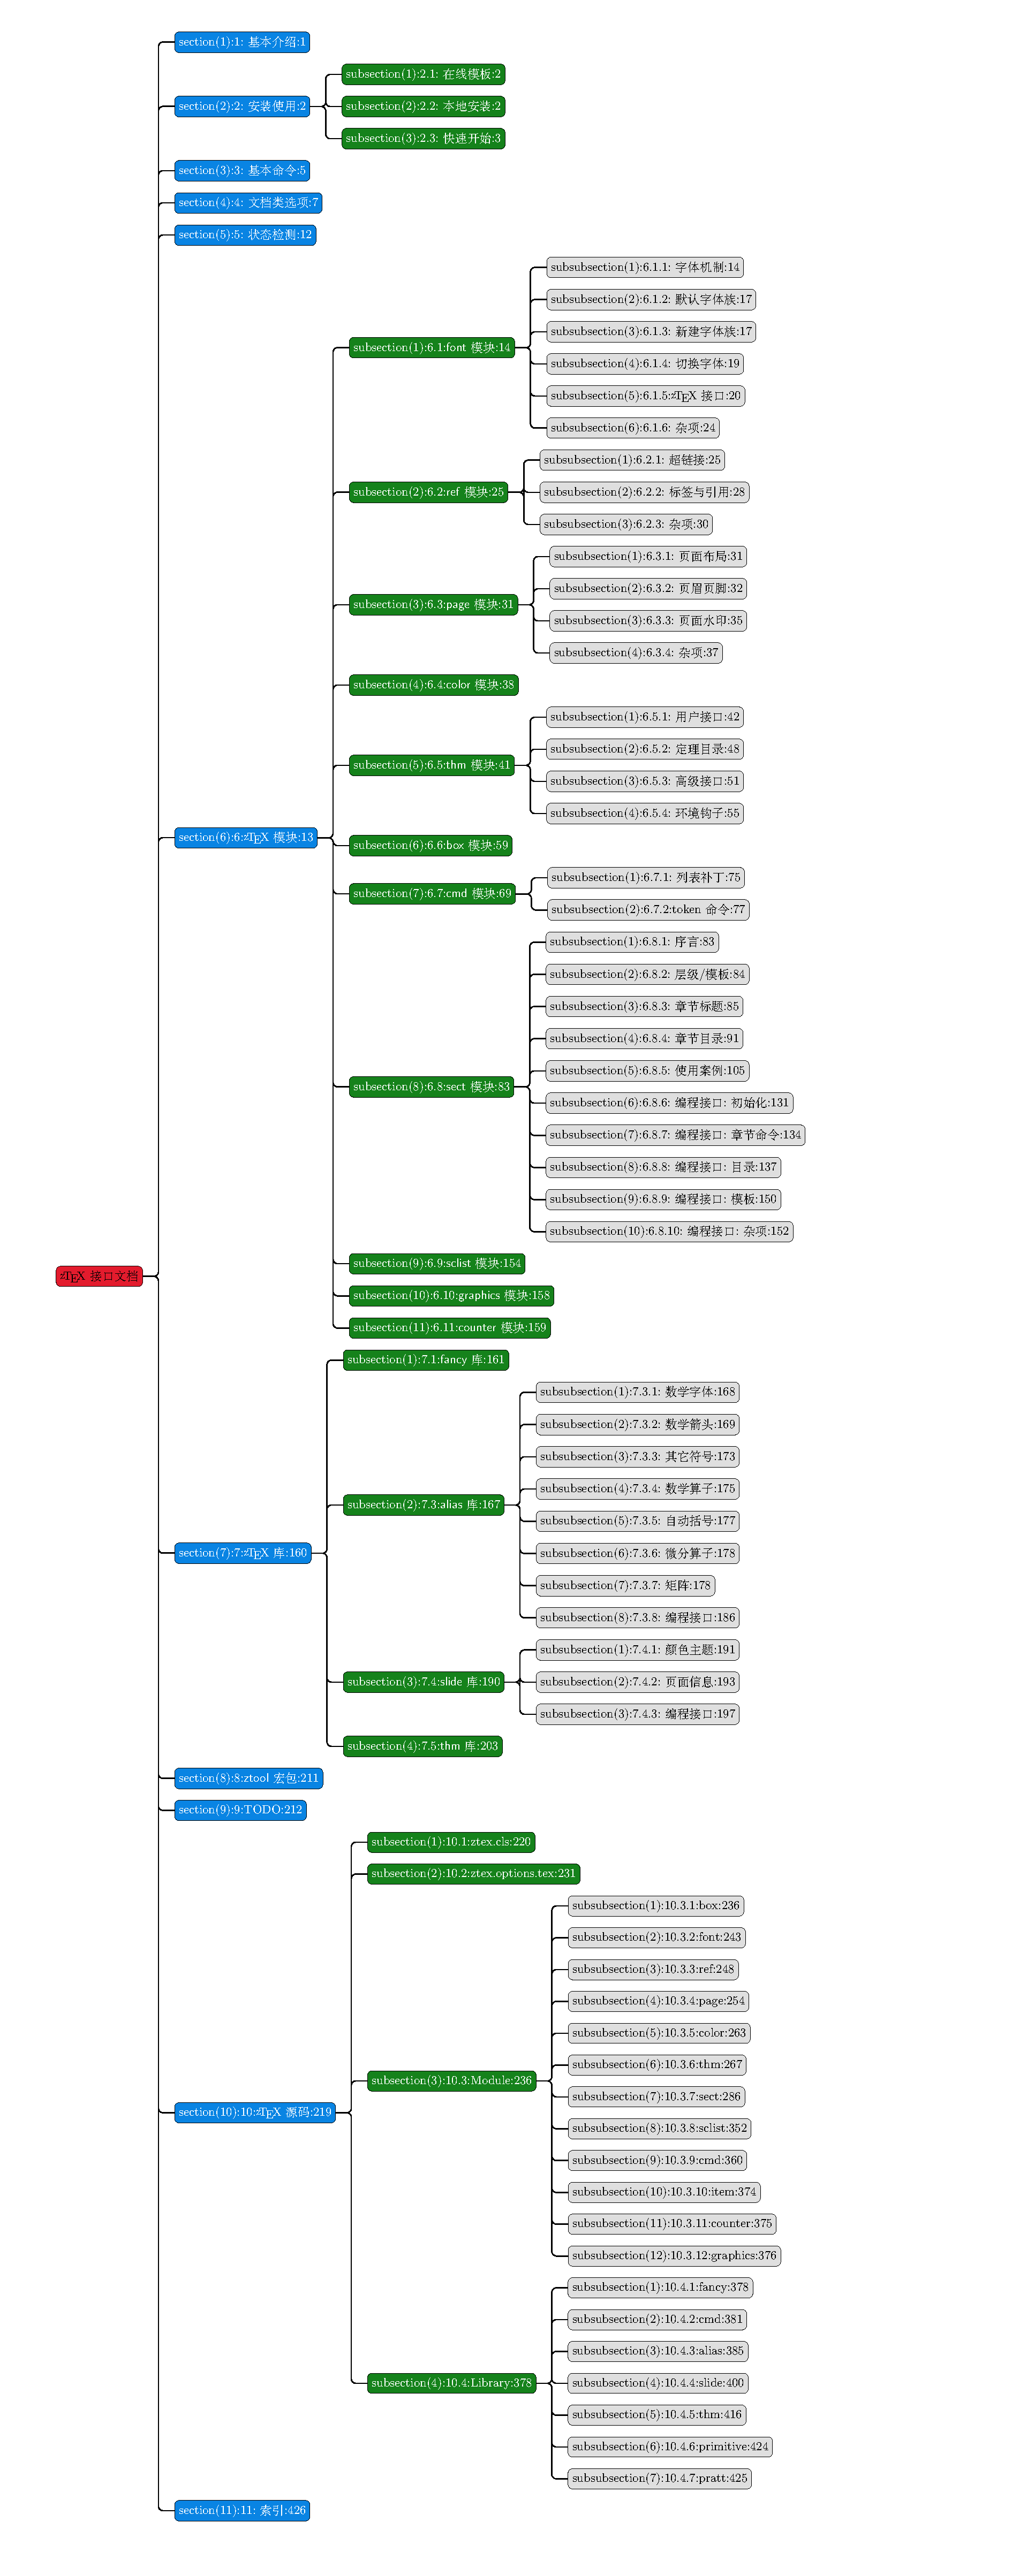
\includegraphics[height=.95\paperheight]{./support/pics/toctree.pdf}
  \vfill\mbox{}
\end{center}
\restoregeometry


\ExplSyntaxOn
\gdef\ztexKeyValParent{\zkeycolor{gray}{\l__codedoc_parent_key_ztex_tl/}}
\ExplSyntaxOff
